\documentclass{standalone}
\begin{document}
	\section{Timing}
	
	One of the highlights of the pipeline is the brief amount of time required to obtain a complete segmentation. In order to characterize this features, I have performed a benchmark on $5$ CR scans with different number of slices. For each scan I have performed separately the lung extraction and the labeling step, repeating the procedure several time. The whole test was performed on the server of the Department of Physics and Astronomy. 
	
	As we have seen, each operation in each script involves the single slice, and it is repeated for the whole scan in the axial direction. as a consequence the time required to segment different scans changes linearly according to the number of slices. In order to measure the time required to performs each operation on each slice I have performed a linear fit and takes the angular coefficient. 
	
	\begin{figure}
		\centering
			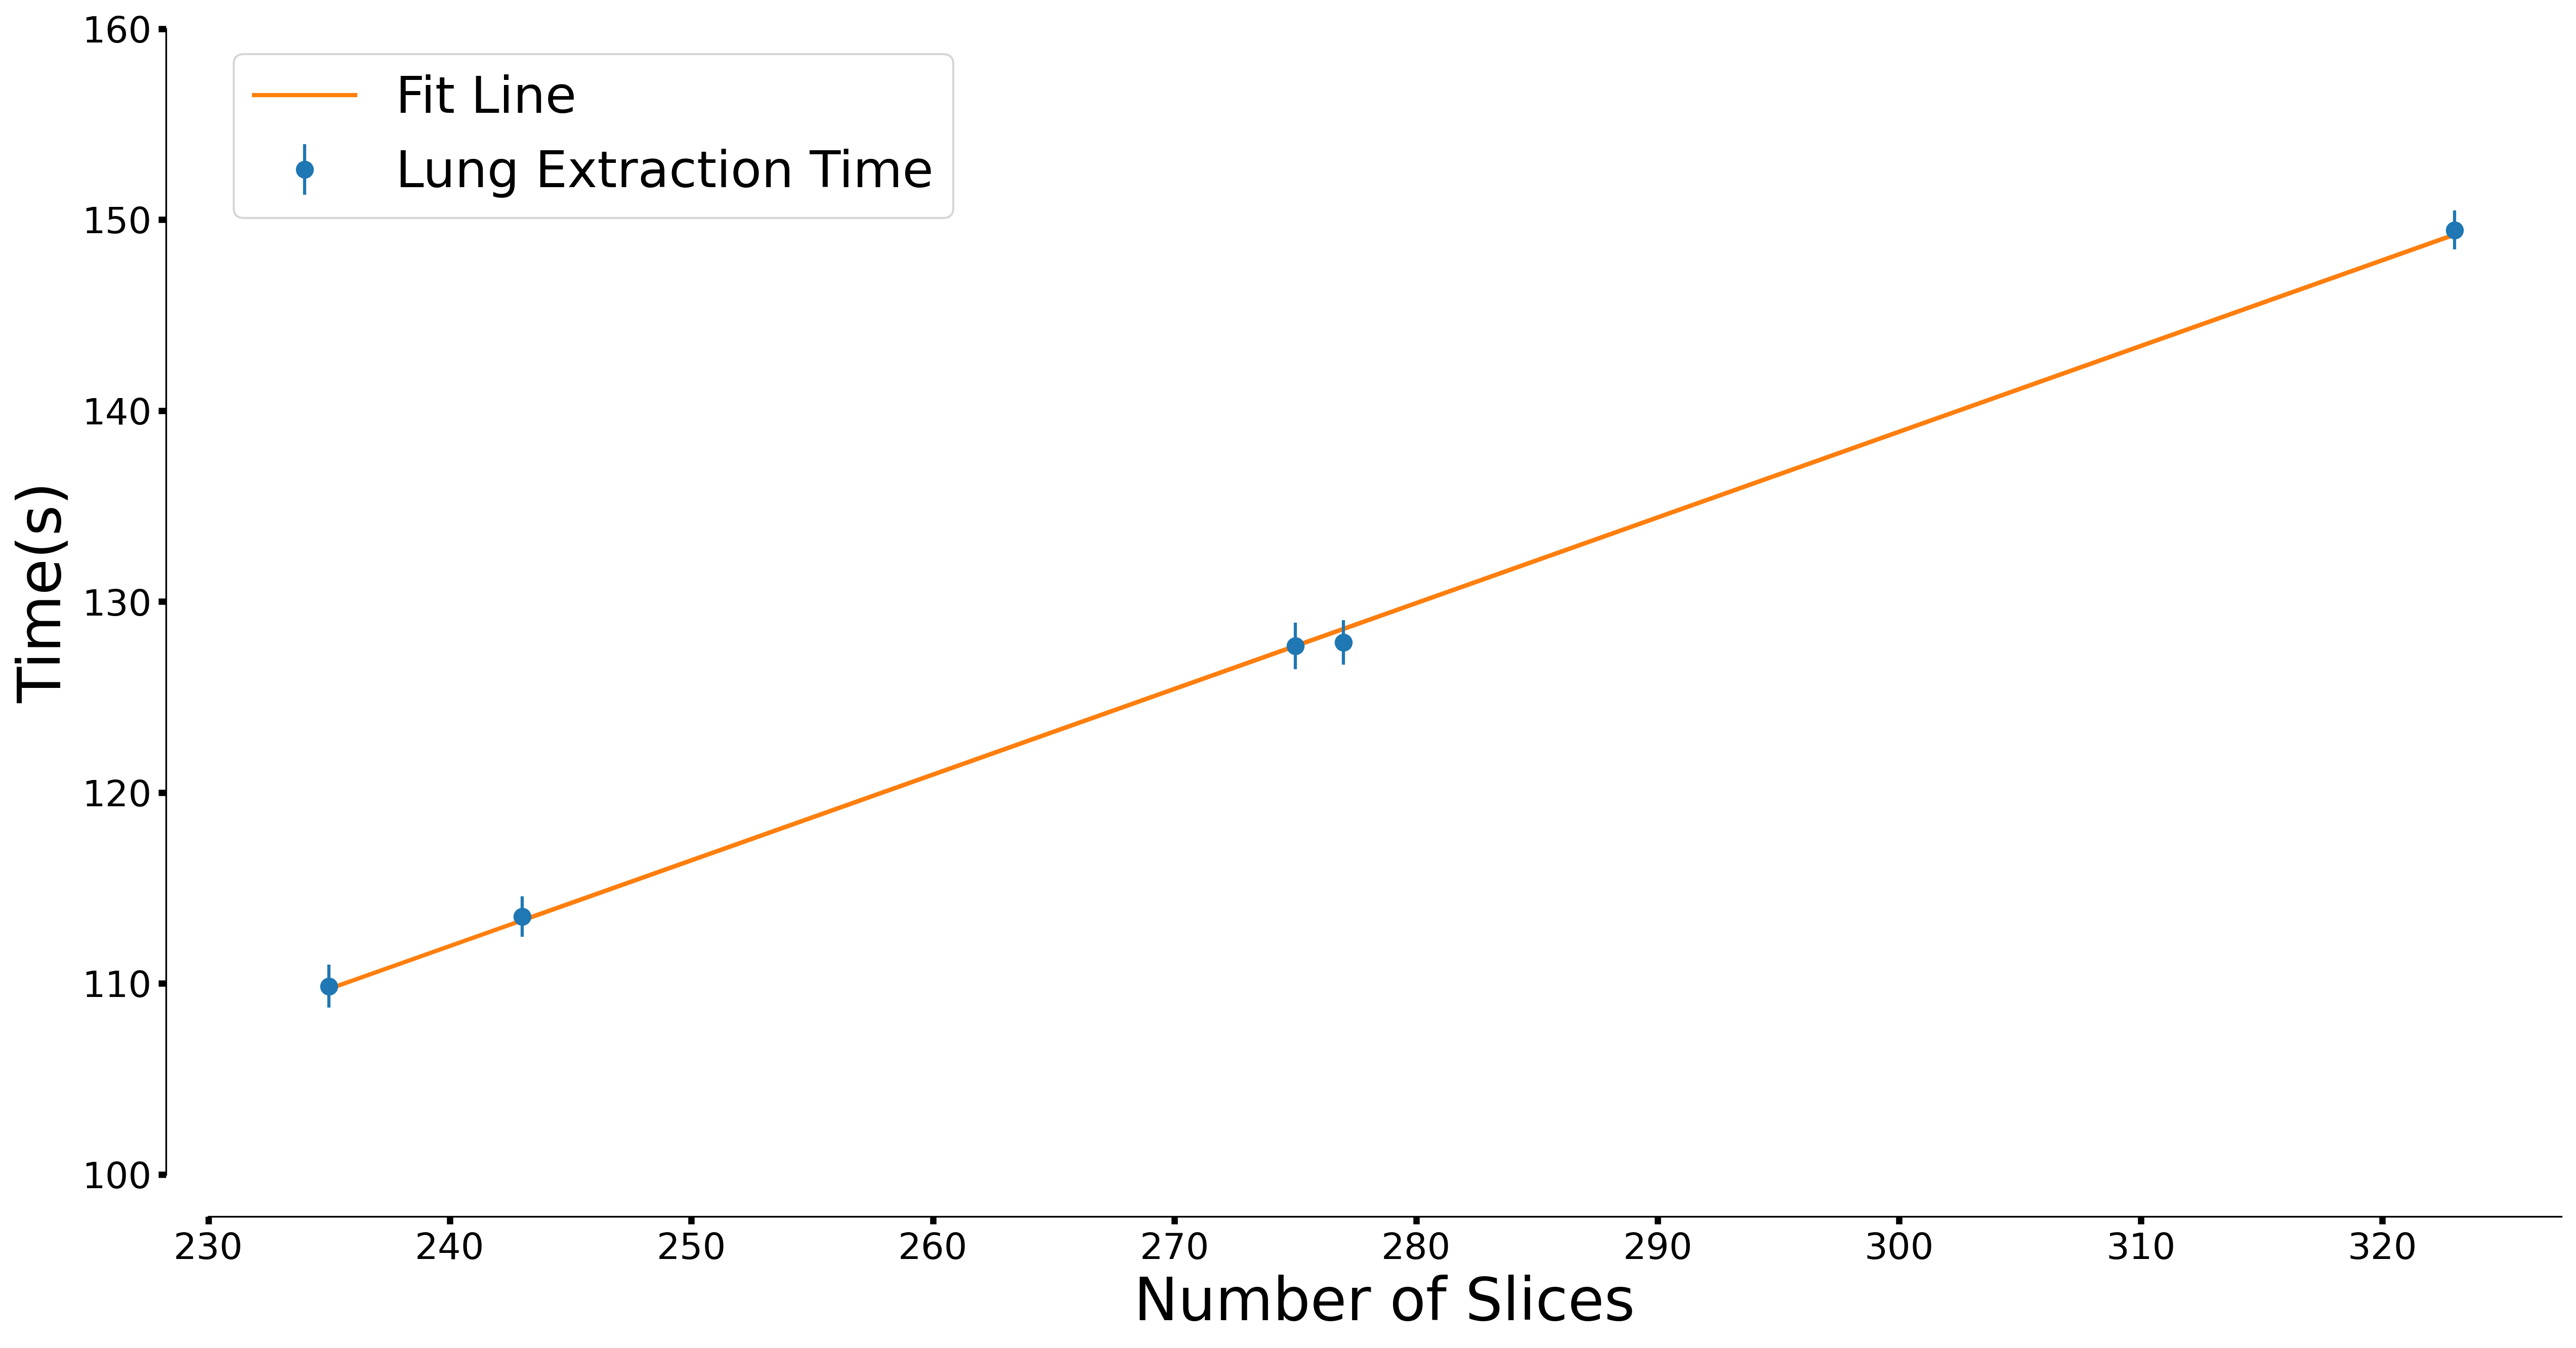
\includegraphics[width=\linewidth]{Lung_timing.png}
			\caption{Lung segmentation time vs number of slice. We can see that the time required to perform the lung segmentation increase linerly with the number of slices. We can also see that in the worst case the lung extraction requires more or less $2$ minutes.}\label{fig:LungTime}
	\end{figure}

	In \figurename\,\ref{fig:LungTime} I have reported the time for the lung extraction as a function of the number of slice in the scan. As we expeted the it has a linear trend. In the worst case It requires $125\,sec$ to perform the lung extraction. With the linear fitting I was able to find the time required to process each slice which tesuts: $449.94\pm 0.03\,ms$. We have to notice that these times are acquired without GPU support. Since the application of the U-Net model is performed by \textsc{torch}, with a suitable hardware it is possible to parallelize the computing and achieve also lower times.
	
		
	\begin{figure}
		\centering
		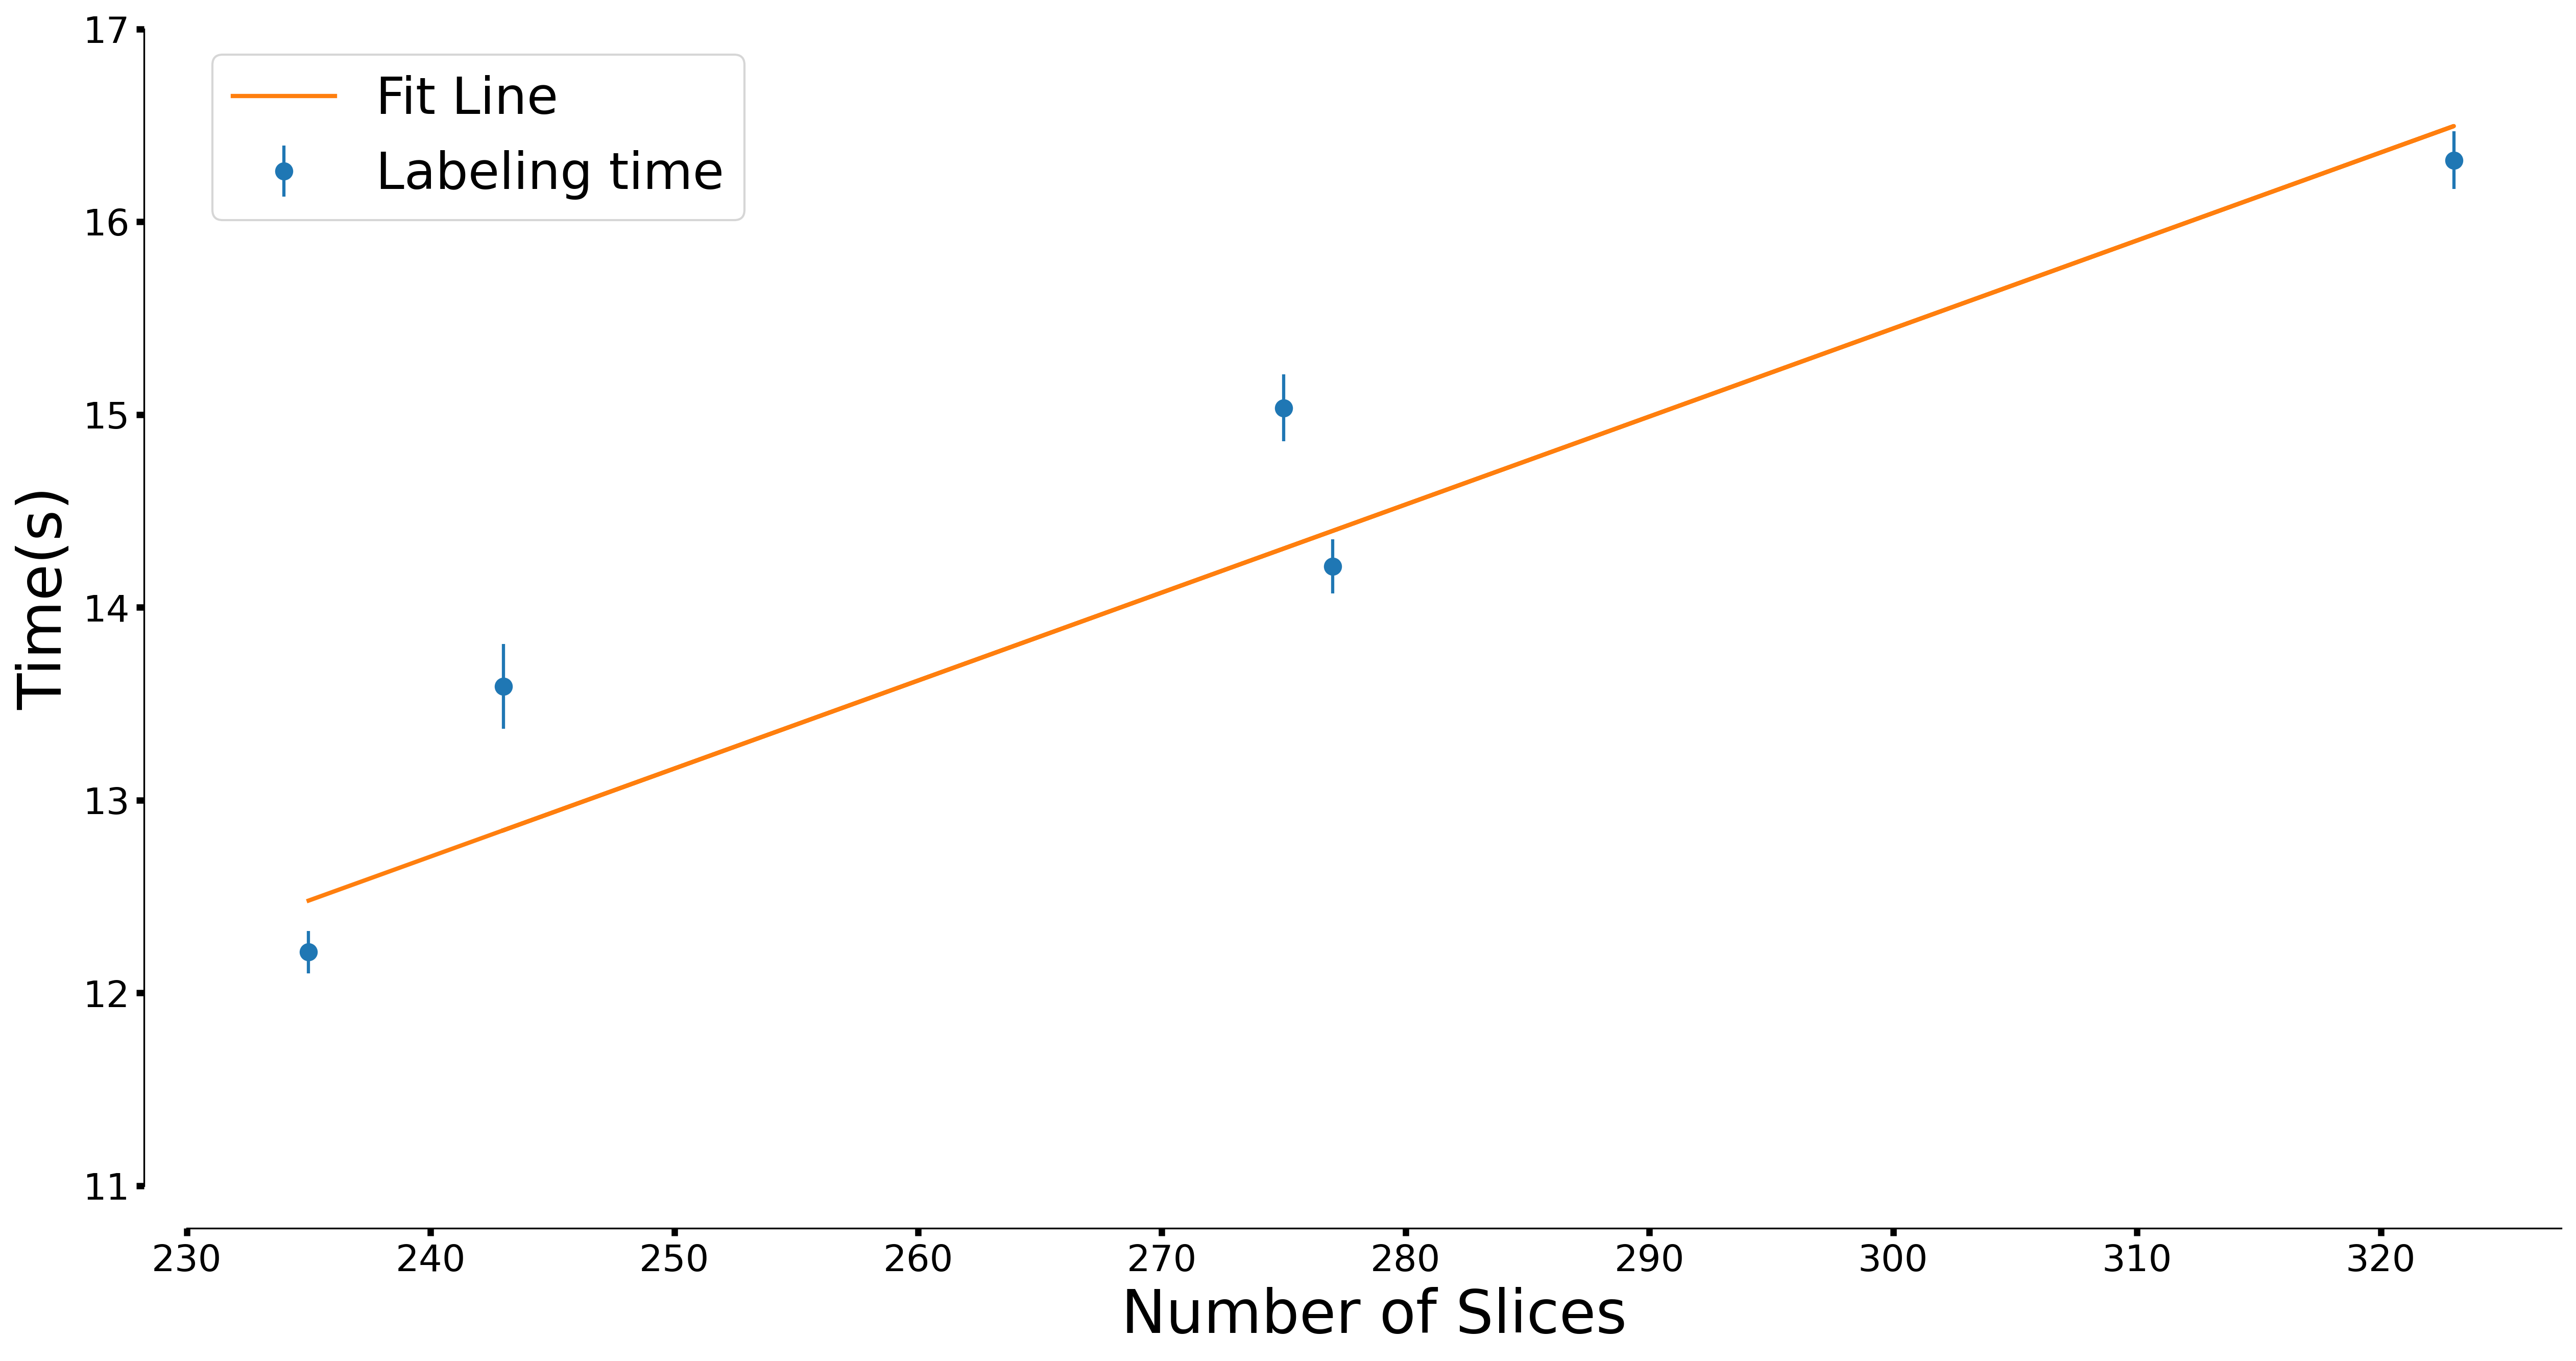
\includegraphics[width=\linewidth]{Labels_timing.png}
		\caption{Labeling time vs number of slice. This time incorporates also the creation of the multi-channel image. As we expected increase linearly with the number of slices and achieve a segmentation in less that $17\,sec$.}\label{fig:LabTime}
	\end{figure}

	In \figurename\,\ref{fig:LabTime} I have reported the results for the labeling. As we can see also in this case the trend is linear and in the worst case requires less that $17\,sec$. As before I have measured the time required to label each slice which results : $45.65\pm0.05\,ms$. 
	
	In the end we have seen that the pipeline achieve a segmentation in a low amount of time, which can be further reduced if a proper hardware is used. 
	 
	 
	 
\end{document}